\documentclass[12pt]{article}
\usepackage{amssymb}
\usepackage{geometry}
\usepackage{graphicx}
\usepackage[colorlinks=true, allcolors=blue]{hyperref}
\usepackage{cite}
\usepackage{wrapfig}
\usepackage{booktabs}
\usepackage{soul}
\usepackage[most]{tcolorbox}
\usepackage{amsmath}
\usepackage{lipsum}
\usepackage{caption}
\usepackage{tabularx}
\usepackage{ulem}
\usepackage{xcolor}
\usepackage{tikz}
\usetikzlibrary{arrows.meta, positioning, shapes}
\usepackage{sectsty}

%--------- Define Colors ---------
\definecolor{titleColor}{HTML}{800000}        % Maroon
\definecolor{sectionColor}{HTML}{4682B4}      % SteelBlue
\definecolor{subsectionColor}{HTML}{6A5ACD}   % SlateBlue
\definecolor{textHighlight}{HTML}{DAA520}     % Goldenrod
\definecolor{backgroundColor}{HTML}{F0F8FF}   % AliceBlue
\definecolor{emphasisColor}{RGB}{200, 50, 50} % ForestGreen

\sectionfont{\color{sectionColor}}       % Color for \section
\subsectionfont{\color{subsectionColor}} % Color for \subsection

%--------- Custom Highlight Commands ---------
\definecolor{lightblue}{RGB}{230, 240, 255}
\definecolor{lightgreen}{RGB}{220, 255, 220}
\definecolor{lightred}{RGB}{255, 230, 230}
\definecolor{lightyellow}{RGB}{255, 255, 200}
\definecolor{darkblue}{RGB}{0, 51, 102}

\newcommand{\bluehighlight}[1]{\colorbox{lightblue}{#1}}
\newcommand{\greenhighlight}[1]{\colorbox{lightgreen}{#1}}
\newcommand{\redhighlight}[1]{\colorbox{lightred}{#1}}
\newcommand{\yellowhighlight}[1]{\colorbox{lightyellow}{#1}}
\newcommand{\blue}[1]{\textcolor{darkblue}{#1}}
\newcommand{\myemphasis}[1]{\textcolor{emphasisColor}{\textbf{#1}}}

%--------- Color Blocks ---------
\newtcolorbox{blockA}{
  breakable,
  colback=blue!5,
  colframe=blue!40!black,
  enhanced,
  boxrule=0.7pt,
  arc=2mm,
  left=4mm,right=4mm,top=2mm,bottom=2mm
}

\newtcolorbox{blockB}{
  breakable,
  colback=red!5,
  colframe=red!40!black,
  enhanced,
  boxrule=0.7pt,
  arc=2mm,
  left=4mm,right=4mm,top=2mm,bottom=2mm
}

\newtcolorbox{blockC}{
  breakable,
  colback=green!5,
  colframe=green!40!black,
  enhanced,
  boxrule=0.7pt,
  arc=2mm,
  left=4mm,right=4mm,top=2mm,bottom=2mm
}

\newtcolorbox{blockD}{
  breakable,
  colback=purple!5,
  colframe=purple!40!black,
  enhanced,
  boxrule=0.7pt,
  arc=2mm,
  left=4mm,right=4mm,top=2mm,bottom=2mm
}

%--------- Title ---------
\title{\textcolor{titleColor}{\textbf{\Huge Supply Chain Analysis and Intelligence for Pharmacy V13 Platform }}}

\author{B. M. Osman\thanks{Al Nahada University, Cairo \\ \texttt{babikerosman@yahoo.com}}}
\date{\today}

\begin{document}
\maketitle
% ============================================================
% SUPPLY CHAIN ANALYSIS AND INTELLIGENCE
% ============================================================
\begin{abstract}

Pharmacy V13 is conceived as an integrated management intelligence system that
transforms routine pharmacy operations into structured, evidence-based
decision support. Rather than functioning solely as a system for recording
medicines, purchases, sales, inventory, suppliers, and financial transactions,
V13 establishes a progressive analytical architecture linking operational
evidence to information, analytical understanding, management intelligence,
and accountable decision-making.

The system incorporates a dedicated Supply Chain Analysis and Intelligence
Layer, supported by the REEM intelligence engine, to integrate observed
purchasing, sales, inventory, supplier, expiry, and demand evidence. Detailed
computational outputs from analytical models are transformed into management
summaries, visual analytics, risk and exception indicators, model-readiness
assessments, and evidence-traceable management signals. The analytical
portfolio includes demand forecasting, stock coverage, ABC analysis, expiry
risk, reorder point, safety stock, economic order quantity (EOQ), and Monte
Carlo uncertainty analysis.

A central principle of the architecture is the distinction between observed
evidence, derived indicators, model outputs, and decision intelligence. Model
execution alone is therefore not considered sufficient for operational use.
Models are assessed according to their analytical purpose and evidence
requirements. Continuous forecasting models are evaluated through forecast
error and residual analysis, optimisation models through parameter and
sensitivity analysis, while appropriate binary classification models may be
evaluated using confusion matrices, precision, recall, sensitivity,
specificity, F1 score, calibration, and receiver operating characteristic
(ROC) analysis with area under the curve (AUROC), where adequate labelled
historical outcomes exist.

The architecture adopts a progressive model-readiness framework ranging from
\textit{Available} and \textit{Partial} to \textit{Ready for Extension} and
\textit{Operationally Validated}. This prevents mathematically completed
calculations from being interpreted automatically as validated procurement
recommendations. Instead, Pharmacy V13 positions analytical models as
transparent instruments for management understanding, risk assessment, and
decision support.

The overall objective is to establish a scientifically defensible and
evidence-traceable pathway from observed pharmacy transactions to reliable
historical knowledge, validated analytical models, risk-aware prediction,
responsible optimisation, and accountable management action. In this
architecture, artificial intelligence and statistical modelling inform
management; they do not replace human judgement or organisational
responsibility.

\end{abstract}

\tableofcontents 


\newpage


\section{Supply Chain Analysis and Intelligence}

\subsection{Overview}

Pharmacy V13 extends its management intelligence architecture through a
dedicated \textbf{Supply Chain Analysis Layer}. This layer connects
operational purchasing, sales, inventory, supplier, expiry, and demand
evidence with analytical models and management interpretation.

The purpose is not to reproduce long model tables. Instead, the system
transforms detailed computational outputs into concise management signals,
visual summaries, analytical diagnostics, and model-assessment information.

\subsection{Supply Chain Intelligence Architecture}

The conceptual flow is:

\begin{center}
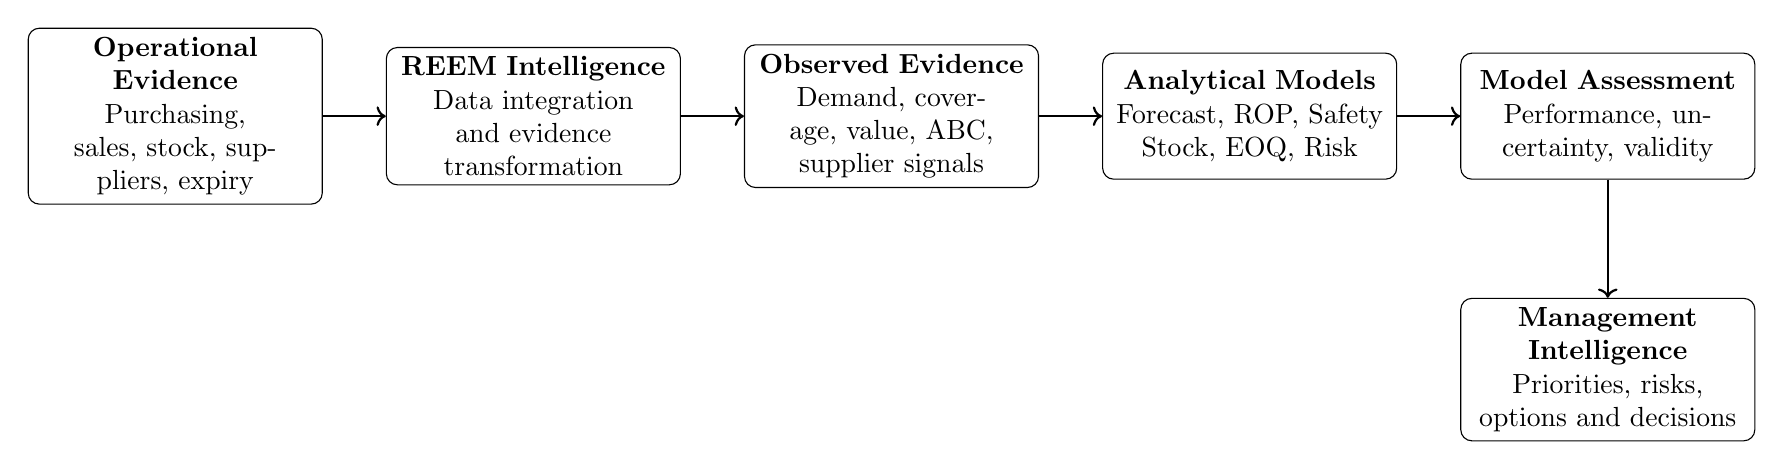
\begin{tikzpicture}[
    node distance=8mm,
    box/.style={
        rectangle,
        rounded corners,
        draw,
        align=center,
        text width=35mm,
        minimum height=16mm
    },
    arrow/.style={->, thick}
]

\node[box] (op) {
    \textbf{Operational Evidence}\\
    Purchasing, sales, stock, suppliers, expiry
};

\node[box, right=of op] (reem) {
    \textbf{REEM Intelligence}\\
    Data integration and evidence transformation
};

\node[box, right=of reem] (obs) {
    \textbf{Observed Evidence}\\
    Demand, coverage, value, ABC, supplier signals
};

\node[box, right=of obs] (models) {
    \textbf{Analytical Models}\\
    Forecast, ROP, Safety Stock, EOQ, Risk
};

\node[box, right=of models] (assessment) {
    \textbf{Model Assessment}\\
    Performance, uncertainty, validity
};

\node[box, below=15mm of assessment] (decision) {
    \textbf{Management Intelligence}\\
    Priorities, risks, options and decisions
};

\draw[arrow] (op) -- (reem);
\draw[arrow] (reem) -- (obs);
\draw[arrow] (obs) -- (models);
\draw[arrow] (models) -- (assessment);
\draw[arrow] (assessment) -- (decision);

\end{tikzpicture}
\end{center}

\subsection{REEM as the Supply Chain Intelligence Layer}

REEM provides the analytical bridge between the operational V13 database and
management-facing supply chain intelligence.

Its conceptual responsibilities include:

\begin{itemize}
    \item integrating purchasing, sales, inventory, supplier, and expiry evidence;
    \item determining the available observation period;
    \item measuring observed demand from actual transactions;
    \item calculating inventory coverage and exposure;
    \item generating preliminary observed-sales ABC analysis;
    \item summarising supplier activity and procurement cost;
    \item identifying data-quality exceptions;
    \item assessing readiness for more advanced analytical models.
\end{itemize}

The REEM layer therefore establishes an important distinction between
\textbf{what the pharmacy has actually observed} and \textbf{what an analytical
model may estimate about the future}.

\subsection{Evidence Status}

Supply chain intelligence should explicitly communicate the maturity of its
evidence.

A conceptual evidence hierarchy is:

\begin{center}
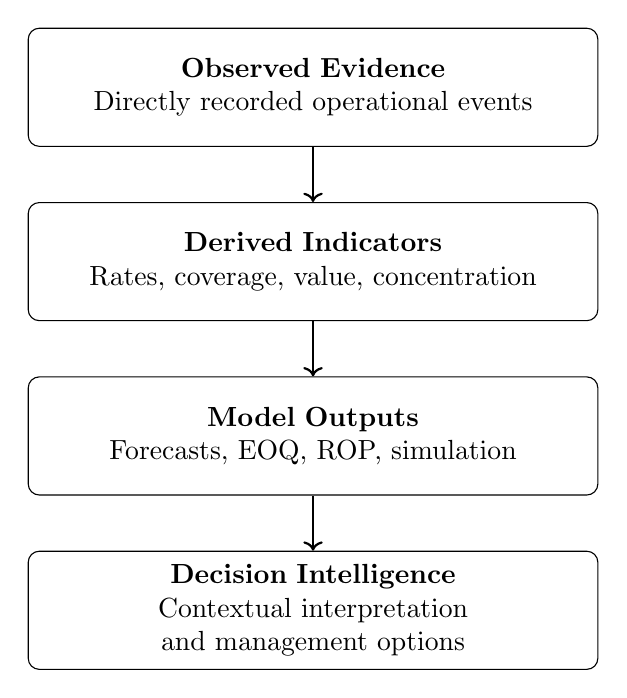
\begin{tikzpicture}[
    node distance=7mm,
    levelbox/.style={
        rectangle,
        rounded corners,
        draw,
        align=center,
        text width=70mm,
        minimum height=15mm
    },
    arrow/.style={->, thick}
]

\node[levelbox] (evidence) {
    \textbf{Observed Evidence}\\
    Directly recorded operational events
};

\node[levelbox, below=of evidence] (indicators) {
    \textbf{Derived Indicators}\\
    Rates, coverage, value, concentration
};

\node[levelbox, below=of indicators] (outputs) {
    \textbf{Model Outputs}\\
    Forecasts, EOQ, ROP, simulation
};

\node[levelbox, below=of outputs] (intelligence) {
    \textbf{Decision Intelligence}\\
    Contextual interpretation and management options
};

\draw[arrow] (evidence) -- (indicators);
\draw[arrow] (indicators) -- (outputs);
\draw[arrow] (outputs) -- (intelligence);

\end{tikzpicture}
\end{center}

The system should never present a model output with greater certainty than is
supported by the underlying evidence.

For example, an EOQ calculation may be mathematically completed while the
model remains only partially validated because ordering and holding-cost
parameters or sufficiently mature demand history are unavailable.

\subsection{Management Summary Rather Than Raw Tables}

Individual Python models may generate large tables containing results for many
medicines. These tables remain useful as computational and audit artefacts,
but they should not be the primary management interface.

The management layer should instead provide:

\begin{itemize}
    \item key aggregate indicators;
    \item ranked exceptions;
    \item top-risk medicines;
    \item concentration and distribution summaries;
    \item concise model-status information;
    \item visual trends and comparisons;
    \item model assumptions and evidence status;
    \item access to detailed analytical results when required.
\end{itemize}

The conceptual transformation is:

\[
\text{Large Model Output}
\rightarrow
\text{Summary}
\rightarrow
\text{Visual Pattern}
\rightarrow
\text{Interpretation}
\rightarrow
\text{Management Attention}.
\]

\subsection{Supply Chain Visual Analytics}

Graphs provide a more efficient representation of large analytical outputs.

Important visualisations include:

\begin{center}

\begin{tabularx}{\textwidth}{p{40mm} X X}
\hline
\textbf{Visual analysis} &
\textbf{Primary measure} &
\textbf{Management purpose} \\
\hline

Demand profile &
Observed demand by medicine or period &
Identify consumption patterns and concentration. \\

Inventory coverage &
Stock relative to observed demand &
Identify potentially excessive or constrained coverage. \\

ABC concentration &
Revenue or consumption value by class &
Show where economic attention is concentrated. \\

EOQ comparison &
Current stock versus calculated EOQ &
Compare current position with the model's economic reference quantity. \\

Expiry exposure &
Quantity or value by expiry horizon &
Visualise time-related inventory vulnerability. \\

Supplier analysis &
Purchase quantity and procurement cost &
Compare procurement activity and supplier contribution. \\

Risk distribution &
Simulated or estimated outcomes &
Show uncertainty rather than relying on a single point estimate. \\

Model performance &
Observed versus predicted outcomes &
Evaluate how well analytical models correspond to subsequent evidence. \\

\hline
\end{tabularx}

\end{center}

Graphs should complement, rather than replace, the underlying numerical
evidence.

\subsection{Analytical Model Portfolio}

The supply chain analytical portfolio includes:

\begin{center}

\begin{tabularx}{\textwidth}{p{38mm} X X}
\hline
\textbf{Model} &
\textbf{Question} &
\textbf{Analytical output} \\
\hline

Demand Forecasting &
What demand may occur during the planning horizon? &
Forecast and associated uncertainty. \\

ABC Analysis &
Which medicines deserve greater management attention? &
Priority classification and concentration analysis. \\

Stock Coverage &
How long could current stock support observed demand? &
Coverage estimate and exception signals. \\

Expiry Risk &
Which inventory may become vulnerable before consumption? &
Expiry exposure and priority signals. \\

Reorder Point &
When should replenishment be considered? &
Replenishment threshold based on demand and lead-time assumptions. \\

Safety Stock &
How much uncertainty protection may be required? &
Buffer estimate based on demand and supply variability. \\

EOQ &
What quantity provides an economic reference under stated assumptions? &
Calculated economic order quantity. \\

Monte Carlo &
What outcomes are plausible under uncertainty? &
Probability distributions and risk scenarios. \\

\hline
\end{tabularx}

\end{center}

These models are complementary. No single model represents the entire supply
chain.

\subsection{Model Assessment and Validation}

A mature supply chain intelligence system must evaluate its models rather than
only execute them.

The conceptual assessment framework is:

\[
\text{Model Calculation}
\rightarrow
\text{Validation}
\rightarrow
\text{Performance Assessment}
\rightarrow
\text{Calibration}
\rightarrow
\text{Operational Use}.
\]

Model assessment may include:

\begin{itemize}
    \item predictive accuracy;
    \item sensitivity and specificity where classification is appropriate;
    \item precision and recall;
    \item F1 score;
    \item calibration;
    \item threshold analysis;
    \item confusion matrices;
    \item residual analysis;
    \item forecast error measures;
    \item sensitivity analysis;
    \item scenario analysis;
    \item uncertainty assessment.
\end{itemize}

\subsection{ROC Curve and Classification Assessment}

ROC analysis is appropriate for supply chain models that classify a future
binary event, such as whether an item will require a replenishment review,
experience a stockout, or enter a defined risk category.

The receiver operating characteristic framework evaluates the relationship
between:

\[
\text{True Positive Rate}
\quad\text{and}\quad
\text{False Positive Rate}.
\]

The area under the ROC curve (AUROC) provides a threshold-independent measure
of discrimination.

However, ROC analysis should \textbf{not} be applied indiscriminately to
continuous optimisation models.

For example:

\begin{center}

\begin{tabularx}{\textwidth}{p{42mm} X}
\hline
\textbf{Model} &
\textbf{Appropriate assessment approach} \\
\hline

Demand Forecasting &
Forecast error, residual analysis, calibration, and prediction intervals. \\

EOQ &
Parameter sensitivity, cost assumptions, and scenario analysis. \\

ROP / Safety Stock &
Service-level performance, stockout behaviour, and sensitivity to demand and
lead-time assumptions. \\

Expiry Risk Classification &
Confusion matrix, precision, recall, and ROC/AUROC where sufficient labelled
outcomes exist. \\

Stockout Classification &
ROC/AUROC, precision, recall, sensitivity, and specificity where historical
outcomes are available. \\

Monte Carlo &
Distribution validation, scenario sensitivity, and comparison of simulated
versus observed outcomes. \\

\hline
\end{tabularx}

\end{center}

Thus, \textbf{model assessment is model-specific}. The architecture should
select the assessment method according to the type of prediction or decision
being evaluated.

\subsection{Model Readiness}

Before a model becomes operationally influential, V13 should assess whether
the necessary evidence and parameters are available.

A conceptual readiness classification is:

\begin{center}

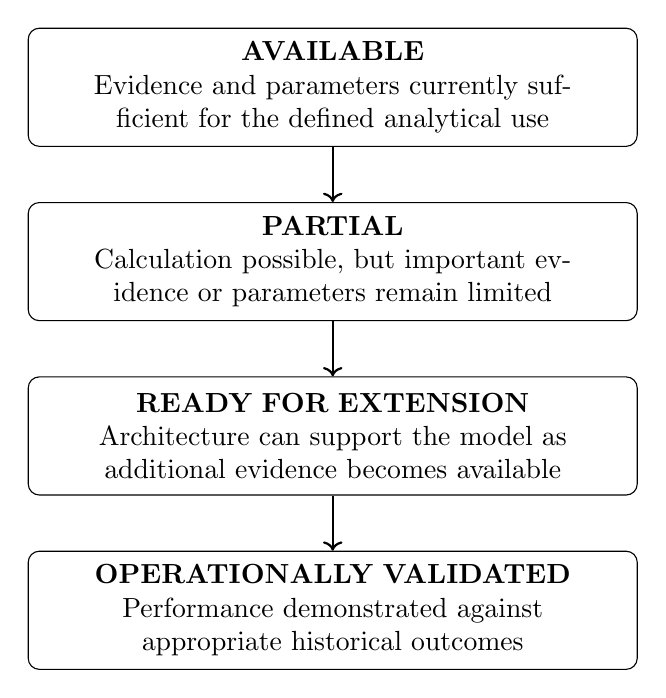
\begin{tikzpicture}[
    node distance=7mm,
    levelbox/.style={
        rectangle,
        rounded corners,
        draw,
        align=center,
        text width=75mm,
        minimum height=15mm
    },
    arrow/.style={->, thick}
]

\node[levelbox] (available) {
    \textbf{AVAILABLE}\\
    Evidence and parameters currently sufficient for the defined analytical use
};

\node[levelbox, below=of available] (partial) {
    \textbf{PARTIAL}\\
    Calculation possible, but important evidence or parameters remain limited
};

\node[levelbox, below=of partial] (extension) {
    \textbf{READY FOR EXTENSION}\\
    Architecture can support the model as additional evidence becomes available
};

\node[levelbox, below=of extension] (validated) {
    \textbf{OPERATIONALLY VALIDATED}\\
    Performance demonstrated against appropriate historical outcomes
};

\draw[arrow] (available) -- (partial);
\draw[arrow] (partial) -- (extension);
\draw[arrow] (extension) -- (validated);

\end{tikzpicture}

\end{center}

This prevents a mathematically valid calculation from automatically becoming
an operational recommendation.

\subsection{Management Interpretation}

Supply chain intelligence should ultimately answer management questions rather
than merely display model outputs.

A management interpretation layer may synthesise:

\[
\text{Demand}
+
\text{Stock}
+
\text{Expiry}
+
\text{Supplier}
+
\text{Financial Exposure}
+
\text{Model Evidence}
\]

to identify areas requiring attention.

For example:

\[
\text{High Expected Demand}
+
\text{Low Coverage}
+
\text{Long Lead Time}
\Rightarrow
\text{Replenishment Attention}.
\]

Conversely:

\[
\text{Low Expected Demand}
+
\text{High Stock}
+
\text{Short Remaining Shelf Life}
\Rightarrow
\text{Expiry Exposure}.
\]

These expressions represent \textbf{management signals}, not automatic
management decisions.

\subsection{Supply Chain Management Cockpit}

The final management-facing supply chain view should therefore move from
detailed computational tables toward a layered cockpit:

\begin{center}

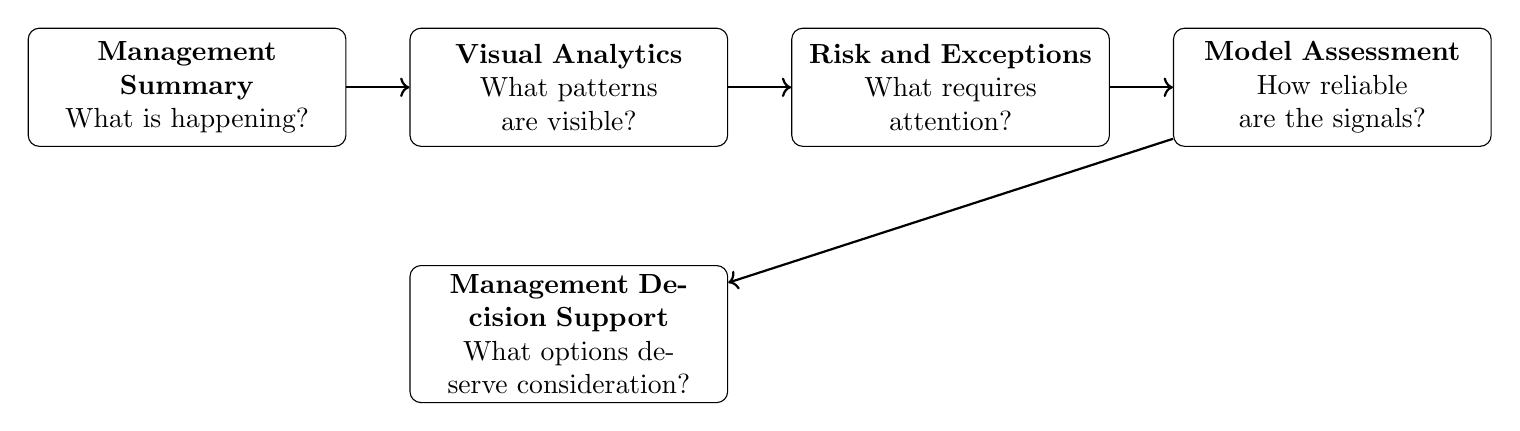
\begin{tikzpicture}[
    node distance=8mm,
    box/.style={
        rectangle,
        rounded corners,
        draw,
        align=center,
        text width=38mm,
        minimum height=15mm
    },
    arrow/.style={->, thick}
]

\node[box] (summary) {
    \textbf{Management Summary}\\
    What is happening?
};

\node[box, right=of summary] (visual) {
    \textbf{Visual Analytics}\\
    What patterns are visible?
};

\node[box, right=of visual] (risk) {
    \textbf{Risk and Exceptions}\\
    What requires attention?
};

\node[box, right=of risk] (assessment) {
    \textbf{Model Assessment}\\
    How reliable are the signals?
};

\node[box, below=15mm of visual] (action) {
    \textbf{Management Decision Support}\\
    What options deserve consideration?
};

\draw[arrow] (summary) -- (visual);
\draw[arrow] (visual) -- (risk);
\draw[arrow] (risk) -- (assessment);
\draw[arrow] (assessment) -- (action);

\end{tikzpicture}

\end{center}

The detailed Python model tables remain available as supporting analytical
evidence, while the management interface presents their meaning in a compact,
visual, and assessable form.

\begin{center}

\fbox{
\begin{minipage}{0.90\textwidth}

\begin{center}
\textbf{Supply Chain Intelligence Principle}
\end{center}

V13 should not ask management to read the model output. It should transform
model output into understandable, assessable, evidence-traceable management
intelligence.

\end{minipage}
}

\end{center}

\subsection{Future Development}

As the historical evidence base grows, the supply chain layer can progressively
move from exploratory analysis toward validated predictive and prescriptive
decision support.

The intended progression is:

\[
\text{Observed Transactions}
\rightarrow
\text{Reliable History}
\rightarrow
\text{Validated Models}
\rightarrow
\text{Performance Assessment}
\rightarrow
\text{Risk-Aware Prediction}
\rightarrow
\text{Optimisation}
\rightarrow
\text{Accountable Management Action}.
\]

This provides a scientifically defensible path from the current operational
system toward a mature pharmacy supply chain intelligence platform.


\end{document} 

